\section{Graph Database} \label{sec:gdb}

A \emph{graph database} (short for \emph{graph database management system}) provides Create, Read, Update, and Delete (CRUD) operations for a graph data model. Graphs, based on the graph theory in mathematics, consist out of \emph{nodes} and \emph{edges}, also often referred to as \emph{relationships}. Both nodes and edges are \emph{first-class citizens} in a graph data model, meaning that they are entities with standard operations that can be performed on them. A graph database actually stores graphs as connected data. This contrasts with other database concepts, where data is implicitly connected and require additional processing to be retrieved. \cite[p.~1,~5,~6,~19]{robinson2015}

% Here I could write about Graph Compute Engines, but naw...
% I could also write about the difference between underlying
% storage vs processing engines \cite[p.~6]{robinson2015}}
% but that is probably not very helpful

The specific graph model used by these systems can vary, the most common form is the \emph{labeled property graph model}. A labeled property graph consists out of nodes and relationships. Both of them can have properties which are stored as key-value pairs. Nodes can additionally have labels, used for categorization and identification. All relationships are directed, named and have a start and end node. \cite[p.~4]{robinson2015} An example labeled property graph is visualized in figure \ref{fig:gdb.graph}.

\begin{figure}[H]
    \centering
    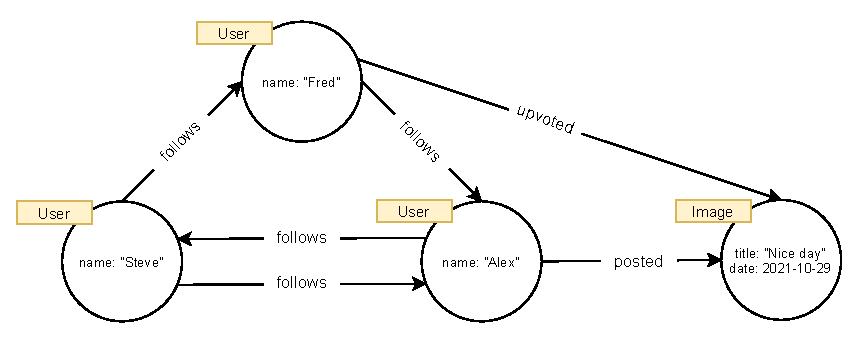
\includegraphics[width=0.9\columnwidth]{res/gdb-graph.pdf}
    \caption{Labeled property graph example}
    \label{fig:gdb.graph}
\end{figure}

Over that past years, several graph database engines for labeled property graphs have been developed. With these multiple query languages have been introduced which vary based on the implementation, expressiveness, purpose and style. The three most common languages \emph{RDF Query Language}, \emph{Cypher} and \emph{Gremlin} all support the same basic operations of \emph{graph pattern matching} and \emph{graph navigation}. \cite[p.~8]{angles2017}

\emph{Basic Graph pattern matching} allows the selection of a node, based on the surrounding graph structure. The query is based on a single node and optionally includes label requirements for selected relationships and nodes. Graph pattern matching can be expanded with additional functionality for projections, unification, optional patterns and determining differences. These functions allow the refinement of searches and increase the precision of results. Basic graph pattern matching with additional features are referred to as \emph{complex graph patterns}. \cite[p.~8,~9]{angles2017}

% "In other words, a bgp for querying an edge-labelled graph is just an edge-labelled graph where variables can now appear as nodes or edge labels;" \cite[p.~9]{angles2017}

The scope of \emph{graph pattern matching} is bound to the described graph structure around a single node. \emph{Graph navigation} allows defining graph patterns for connected nodes and further navigation. The navigated path between nodes can have an arbitrary length. \cite[p.~21,~22]{angles2017} 

